\documentclass[twocolumn, a4paper, uplatex]{UECIEresume}

\usepackage[dvipdfmx]{graphicx}
\usepackage{graphicx}
\usepackage{amsmath}
\usepackage{txfonts}
\usepackage{array}
\usepackage{url}

\title{自然言語処理によるフェイクニュース判断の自動化}
\date{平成 30 年 9 月 25 日}
\affiliation{総合情報学科 メディア情報学 コース}
\supervisor{大須賀 昭彦 教授, 田原 康之 准教授, 清 雄一 准教授}
\studentid{1510151}
\author{栁 裕太}
\headtitle{平成 30 年度 総合情報学科 卒業論文中間発表}
%\headtitle{平成 yy 年度 総合情報学科 卒業論文発表}
%\headtitle{平成 yy 年度 総合情報学科 修士論文中間発表}
%\headtitle{平成 yy 年度 総合情報学科 修士論文発表}

\begin{document}
\maketitle

\section{はじめに}
\subsection{背景}
インターネット環境の浸透により、フェイクニュースの急速な拡散が大きな社会問題として近年取り沙汰されている。
主に人々の扇動を目的に作られたフェイクニュースは、受け手に専門知識がない場合判断が難しい。
そこで有識者が発信された情報の信頼性を判断・公表するファクトチェックが主に米国で盛んになっている状況である。
しかしながら新たに発信される情報とファクトチェックには時間差があるため、
その間に拡散されてしまう状況となっている。

\subsection{先行研究}
過去の先行研究でフェイクニュースを始めとする情報の信頼性判断の研究事例がある。

まず、事前の調査で明らかとなった情報の信頼性が高いwebサイトの特徴をベースに判断する手法\cite{fuk}がある。
ただその調査のデータが古く、現在のwebサイトに当てはめるには少々無理が生じる状況となっている。

また、情報が拡散された経緯をグラフマイニング技術によってフェイクニュースを判断する手法\cite{foot}もある。
こちらはまだ研究が浅く、データセットの入手も少々難しい状況である。

過去のファクトチェック結果による機械学習モデルを構築することで、
新たに発信されるフェイクニュースに対応する研究も行われている\cite{nb}\cite{gilda}。
しかしながら、精度に関しては未だ大きな改善の余地を残しているほか、
使用されたデータセットの信頼性に疑問が残るケースもある。
更に実際に機械学習手法を運用する場合を想定したシステムに関して、未だ有効な提案がないのが現状である。

\section{課題}
課題として挙げられるのは、以下の2点である。
\begin{itemize}
  \item 機械学習によるファクトチェックの精度向上
  \item 新たなニュースとファクトチェック結果が出るまでの時間差
\end{itemize}
特に後者では、ファクトチェック機関の調査が終わるまで少々の時間差があるため、
ファクトチェック結果が公表されても浸透しないというケースが起こりやすい。
そこで信頼性を自動算出・公表することで、
ファクトチェックが終わるまでの間にフェイクニュースの拡散に足止めをかけることを考えた。

この課題を解決するために、\textbf{自動ファクトチェックシステムを構築}することを考えた。
これはSNS上での運用を想定しており、信頼性に疑いがある情報に対して警告を出す形を想定している。

\section{現在の進捗}
\subsection{データセット}
この分野の研究には、発言引用と真偽の要素を併せ持つデータセットが必要である。
使用したのは、ファクトチェック機関politifact.comのファクトチェック結果からなる
LIAR datasetを使用した\cite{pants}。
LIAR dataset掲載の真偽データはpolitifact.comの評価方法"Truth-O-Meter"に準拠\cite{pants}しており、
真偽の度合いによって
"True", "Mostly True", "Half True", "Mostly False", "False",
そして不正確かつばかばかしい主張を示す"Pants-on-Fire"までの7段階評価となっている\cite{truth}。

今回の実験では、自然言語処理によってどれだけ正確に信頼性を自動で判定することができるか調べたものとなっている。

\subsection{予備実験}
全体の流れとしては、以下の図\ref{fig:nagare}の通りである。

\begin{figure}[h]
  \begin{center}
    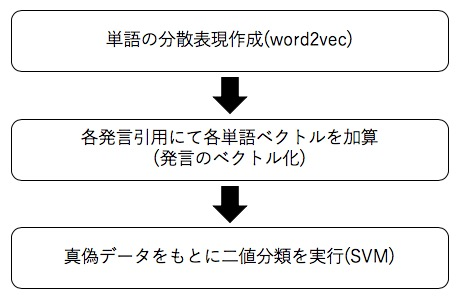
\includegraphics[width=8cm]{fig1.jpg}
    \caption{予備実験の流れ図}
    \label{fig:nagare}
  \end{center}
\end{figure}

まずは全体データセットの発言引用を元にword2vec(gensim)による単語の分散表現を作成する。
その次に各発言内にて、発言がもつ各単語ベクトルを加算・正規化することで、発言のベクトル化を行う。
最後に、各発言ベクトルと真偽を元にSVM(scikit-learn)で教師あり学習・検証を実行する。


LIARデータセットの真偽値に関しては、"Pants-on-Fire"〜"Mostly-False"をFalse、
"Half-True"〜"True"をTrueとして扱った。
なお、その場合の全体件数はTrueは5657件, Falseは7134件だった。

5分割交差検定を行った結果が以下の表\ref{tb:result}の通りである。

\begin{table}[h]
  \begin{center}
    \caption{予備実験結果}
    \label{tb:result}
    \begin{tabular}{l c c c}
      \hline
      手法 & Precision & Recall & F1 score \\
      \hline
      Baseline & 0.557736 & 1.000000 & 0.716085\\
      Proposed method & 0.723439 & 1.000000 & 0.839530\\
      \hline
    \end{tabular}
  \end{center}
\end{table}

Precision(適合率)は全体でのモデルの正答率、
Recall(再現率)はTrue全体内でのTrue看破率を表し、
F1 score(F値)は上記2値の調和平均を表す。
Baselineとして、全てTrueと判断した場合の数値も併記した。

この結果より、word2vec+SVMの手法はBaselineと比較して良好な分類成績を示すことが判明した。
しかしながら、Precisionに関しては改善の余地が残された。

\section{今後の展望}
今回の実験の結果を受け、今後さらなる精度向上に向けた手法の検討を継続する。

また今後は、このフェイクニュース検出システムを実際のSNS上で運用する場合を想定したモデル作りが必要である。
そのために対象となる情報を選定することと、検証方法を考案する必要がある。

ところで、今回扱ったデータセットは全て英語・米国における情報だった。
もしもこれを日本語で運用することを考えた場合、
日本語でLIAR datasetとほぼ同じ情報形式を持つデータセットが必要である。
そのためには日本における第三者機関によるファクトチェックの活発化が求められるが、
残念ながらそのような運動があまりみられないのが現状である。

{\small
\begin{thebibliography}{*}
  \bibitem{fuk}福島隆寛, 内海彰. \textit{Web ページの信頼性の自動推定.} 知能と情報 19.3 (2007): 239-249.
  \bibitem{foot}Wu, Liang, and Huan Liu. \textit{Tracing fake-news footprints: Characterizing social media messages by how they propagate.} Proceedings of the Eleventh ACM International Conference on Web Search and Data Mining. ACM, 2018.
  \bibitem{nb}Mykhailo Granik, Volodymyr Mesyura. \textit{Fake news detection using naive Bayes classifier.} UKRCON(2017):900-903.
  \bibitem{gilda}Shlok Gilda. \textit{Evaluating machine learning algorithms for fake news detection.} SCOReD(2017):110-115.
  \bibitem{pants}Wang, William Yang. \textit{"liar, liar pants on fire": A new benchmark dataset for fake news detection.} Proceedings of the 55th Annual Meeting of the Association for Computational Linguistics (Volume 2: Short Papers)(2017):422-426.
  \bibitem{truth}Angie Drobnic Holan. \textit{The Principles of the Truth-O-Meter: PolitiFact’s methodology for independent fact-checking.} \url{https://www.politifact.com/truth-o-meter/article/2018/feb/12/principles-truth-o-meter-politifacts-methodology-i/}. (Viewed:Sep. 18, 2018).
\end{thebibliography}
}
\end{document}
